\section{Einführung}
Mit der Vorstellung diverser teilautonomer Fahrzeuge in den vergangen Jahren \textit{(Waymo, Uber, Tesla, uvm.)} fängt ein neues zeitalter der Automobilindustrie an. Neu entstehende Seitenmärkte wie Carsharing werden an Wichtigkeit gewinnen, es werden vermutlich weniger Autos benötigt als zur Zeit registriert sind und der Straßenverkehr gewinnt durch diese Autos an Sicherheit. Nun ist ein \textit{autonomes} Auto aber nicht immer gleich ein überall selbstständig fahrendes Auto, sondern es werden immer wieder Updates benötigt, ähnlich zu den Apps auf einem Smartphone. Stellen sie sich dazu das folgende Szenario vor:\\\\
Es ist das Jahr 2030 und wie andere in der Nachbarschaft, haben Sie sich ein autonomes Fahrzeug der Stufe 4 zugelegt. Dies bedeutet, dass ihr Auto in bestimmten Anwendungsfällen die komplette Steuerung übernehmen kann und Sie sich entspannen können. Sie veranstalten mit ihrem neuen Wagen eine Reise nach England und Vergessen, dass der Verkehr dort Links verläuft. Sie würden aber auch gerne in England autonom Fahren, aber ohne eine passende Software ist die nicht möglich. Was nun?\\
Sie benötigen eine Möglichkeit, ein Softwareupdate für ihr Fahrzeug Orts- und zeitunabhängig durchzuführen, damit dieses daraufhin wieder selbstständig fahren kann. Das Auto muss hierzu identifizieren, welche Software es benötigt und soll diese nach Einwilligung von Ihnen installieren. Anschließend ist ihr Auto wieder in der Lage eigenständig zu Fahren und Sie setzen Ihre Reise fort.\\
Dieses Szenario beschreibt eine möglicherweise klassische Situation, die einem in Zukunft in Autos passieren könnte. Durch die unterschiedlichen Fahrbedingungen weltweit ist es schwer denkbar, zu einem Zeitpunkt in naher Zukunft vollständige Autonomie zu erreichen. Stattdessen sollten sich Autos an ihre Umgebungsbedingungen anpassen, um somit den Großteil ihrer alltäglichen Strecken autonom zurückzulegen.\\\\
Diese Arbeit hat das Ziel, zu beachtende Schritte entlang dieses Ablaufs zu identifizieren und zu beschreiben, um somit abschließend eine Wertschöpfungskette zu schaffen. Diese soll als Orientierungshilfe für die Entwicklung derartiges Systeme dienen.\\\\
Um eine Wertschöpfungskette für die Bereitstellung solcher Software zu erstellen, bedarf es einiger Wissensgrundlagen \& Design-Richtlinien welche bei der Erarbeitung einer Wertschöpfungskette stetig beachtet werden müssen aber auch Tools und Methodiken des Wissenschaftlichen Arbeitens.\\
Wandel der GMs\\
neue Seitenmärkte\\
einer davon Bereitstellung neuer Fahrfunktionen\\
Auto soll erweiterbar sein -> Freut den nutzer\\
irgendwie müssen mehrwerte geschaffen werden\\
überall auf der Welt sind Straßen anders ( Apshalt, Dreck, eis, uvm.) -> ein Modell für komplette Welt scheint schier zu groß\\
Auto muss ja nciht 'überall' fahrne können ->doch! Wenn autonome Fahrzeuge gewöhnlich werden, sind vor allem lange autofahrten sehr gut Vorstellbar aufgrund des neuen Komforts\\
\subsection{Altes Kapitel \textit{Zweck und Zielsetzung der Arbeit}}

Hier mal ne State-of-the-Art Anaylse zu autonomen Fahrzeugen schreiben

Die Geschichte der Automobilindustrie geht zurück bis in das späte 19. Jahrhundert. Seit dem hat sich das Automobil als solches sehr stark weiterentwickelt, hin zu dem was wir heute kennen. Mit der Zeit hat sich das Fahrgefühl in Fahrzeugen immer weiter gesteigert. Die ist nicht zuletzt auch zum Dank von multiplen Assistenzsystemen, die heute schon nicht mehr weg zu denken sind. Zum Beispiel der Tempomat, das ABS, der Bremsassistent und viele mehr. Mit Visionären wie Tesla, Uber, Waymo aber mittlerweile auch anderen Teilen der Automobilindustrie, haben sich Fahrzeuge auch zuletzt stetig weiter entwickelt. \\ 
Die Automobilindustrie als solche hat sich aber in ihren Grundzügen kaum weiterentwickelt - bis jetzt. In der Vergangenheit hat ein Automobilhersteller fertige, immer gleiche Autos hergestellt und diese dann verkauft. Laut Juergen Daunis, dem Vize Präsidenten für "Global Sales Connected" bei Ericsson, wird sich dies in den kommenden Jahren ändern.So behauptet er, dass das Produkt "Auto" an Wertschöpfung für den Menschen verlieren wird und die Mehrwerte von Autos eher aus der Unternehmensumwelt, von Dritten kommen werden.\cite{b1} Nun ist schwer Vorstellbar, dass der Großteil an Mehrwerte in Zukunft von Drittanbietern kommen wird. Was aber sicher ist: Es werden viele neue Seitenmärkte im Rahmen von Autonomen Fahrzeugen entstehen. Einer dieser Märkte ist das Verteilen von Software(-Updates) für intelligente Fahrzeuge sein. Dies können Erweiterungen/Verbesserungen für Fahrumfänge sein aber auch Denkbar sind Komfort-Produkte. Diese Updates sollen Orts- \& Zeitunabhängig erfolgen können und somit ein angenehmeres Nutzererlebnis schaffen als heutzutage (Fahrzeughalter müssen für Updates in die Werkstatt).\\
So ist es das Ziel meiner Arbeit, ein (technisches) Grundkonzept für diesen Softwarevertrieb zu schaffen und dabei die essenziellen Komponenten der dabei entstehenden Wertschöpfungskette zu identifizieren. Dieses Grundkonzept soll die Sicherheit von intelligenten Fahrzeugen der Stufe 4 steigern als auch eine mögliche Zukunft der Automobilbranche aufzeigen.\\
\subsubsection{Altes Kapitel: Die Idee}
Mit den ersten autonomen Fahrzeugen bereits heute schon auf dem Markt, steigt die Diskussion um eben diese. Immer mehr Menschen zeigen ernsthaftes Interesse an dieser Art Fahrzeuge und dass, obwohl noch viel zu erforschen ist. Die aktuellen Fahrzeuge sind in sich abgeschlossene, sehr intelligente Systeme, welche Entscheidungen selber treffen. Um die Sicherheit von Fahrzeugen in der Zukunft zu erhöhen, werden diese wohl möglich untereinander kommunizieren können. Die dafür nötige Kommunikationsschnittstelle Sicher, aber vor allem Standardisiert entlang der Automobilindustrie sein. Hinzu kommt, dass nun mal nicht überall auf der Welt immer Autos fahren werden - Fahrzeuge werden also auch in der Zukunft noch Entscheidungen selber treffen können müssen. Wenn man zusätzlich noch die Geschichte des Straßenverkehrs hinzuzieht fällt auf, dass immer wieder neue Herausforderungen für Fahrer entstehen. Sollen also die Autos der Zukunft sicher sein, benötigen sie nicht nur Updates bestehender Software, sondern möglicherweise auch Software für neue, bis jetzt nie da gewesene Situationen. Standardmäßig wird ein Fahrer von seinem Auto 'einfach' gebeten die Steuerung zu übernehmen wenn die Sicherheit nicht gewährleistet werden kann - wenn aber nun immer wieder die gleiche Situation auftaucht und der Fahrer immer wieder übernehmen muss, wird es Zeit für neue Software. Anderseits wäre das 'autonome Fahrzeug' halt nicht mehr so autonom wie vorher, was natürlich vom Kunden als Negativ angesehen wird.\\
Die Idee hierbei ist also, Fahrern passende Software für Problemsituationen anzubieten. Dieser Vertrieb soll nicht nur nach Push-Prinzipien\cite{b2} der Hersteller gehen, sondern der Fahrer soll auch Software selbstständig Suchen sowie orts- und zeitunabhängig Kaufen können. Durch ein derartiges Konzept soll ein Fahrzeug in der Zukunft neue Software erhalten, ohne dazu extra in die Werkstatt zu müssen aber dennoch eine garantierte Fahrsicherheit haben. Außerdem: durch autonomes Fahren ändert sich auch das Verhältnis des Fahrers zum Auto. Mögliche Comfort-Features, genauer gesagt Software-basierte Features, können so auch Vertrieben werden.\\
Jedoch gibt es dabei ein Problem: durch die Vielzahl an Automobilherstellern ist es schwer möglich, einen zentralen Shop für jede existierende Software zu haben. Betrachten wir hierzu Volkswagen: Das Unternehmen selber, bewirbt zum jetzigen Zeitpunkt 18 unterschiedliche Fahrzeugmodelle.\cite{b3} Ausgehend davon, dass die Architektur dieser Fahrzeuge in sich unterschiedlich ist, müsste also entweder eine Software für jedes Modell entwickelt werden, oder eine Software die so modular ist, dass sie auf unterschiedlichste Architekturen anpassbar wäre. Wenn Software zusätzlich noch für andere Tochtermarken verfügbar sein soll, steigt die Komplexität der Thematik enorm, weshalb ich diesem Problem in einem eigenen Kapitel entgegen treten werde. \\
Dieser 'zentrale Shop' ist nötig, da eine Person in der Regel nicht nur Autos einer Marke fährt, die von ihm gekaufte Software aber dennoch immer bei sich haben möchte.\\
\subsection{Wandel der Automobilbranche}
Früher: wirtschaftlicher Wandel
wirtschaftlicher Wandel -> jetzt überfluss an Waren; Um Kunden für sich zu gewinnen hat der Aspekt Qualität wieder an Wichtigkeit gewonnen, was auch Features etc. betrifft. Der Standard der Gesellschaft ist im generellen gestiegen, weshalb in Zukunft wieder Abgrenzung durch etwas nötig ist.\\
aktuell in automobilindustrie Massenproduktion -> wenn autos iun Zukunft modular\\ anpassbar sind, ist kaufrate ggf. geringer (?) -> finde ich hierfür eine Quelle\\
es werden zuj viele Autos für zu wenige Menschen (die es sich liesten können) produziert\\
zu viele autos haben auch zu den Problemen der Neuzeit geführt: Lärm, schlechte Luft, Ressourcen, Tode durch ein Auto\\
Märkte sind immer Nutzergrtriebener; Durch SOcialMedia können sich negativ schlagzeilen zu unternehmen sehr schnell bilden, diese müssen dementsprechend vorsichtiger sein und auf Kunden eingehen\\
Seitenmärkte: Batteriewechsel zum ersetzen des tankens (Better Place: battery Swap); Frühstück/Essen im auto bestellen und durch drivethrough fahren lassen; Auto nicht selber besitzen\\
automobilindustrie hat höhepunkt erreicht und steht möglicherweise vor Fall des bisherigen, klassischen Gechäftsmodells -> hierzu Verkaufszahlen von Automobilherstellern der letzten 2 Jahrzehnte untersuchen\\
Auto zählt immer weniger als Statussymbol sondern als must-have -> In Zukunft ist die Nützlichkeit eines Autos entscheidend, bzw. der Grad zu dem es den Fahrer beim bewältigen von alltäglichen AUfgaben unterstützt (ähnlich zum Smartphone) -> dahin bewegt sich die moderne Welt momentan sowieso (Smarthome, Assistenten, Automatisierung, Ubiquitousy computing, Orts und Zeitunabhöngigkeit -> alles hat die Lebensqualität des Individuums gesteigert\\
Automobilbranche muss nicht zwanghaft dem Umwurf des bisherigen BusinessModels ausgesetzt sein, da die branche sehr politisiert ist und etwas derartiges bereits präventiert worden sein kann.\\
Paris AutoLIB approach -> recherchieren\\
Rishi, S.; Stanley, B. and Gyimesi, K. (2008) Automotive 2020: Beyond the
chaos, Somers, NY: IBM Institute for Business Value.\\
von klassischen bm hin zu service-based business Model -> Masterarbeit aus schweden\\
Probleme/Folgen, die normale Autos verursacht haben.\cite{b19}
\begin{itemize}
	\item Hohe Anzahl an Unfällen
	\item Zu viele Autos ->\\
	https://de.statista.com/statistik/daten/studie/244999/umfrage\\/weltweiter-pkw-und-nutzfahrzeugbestand/\\
	https://de.statista.com/statistik/daten/studie/151749/umfrage\\/entwicklung-der-weltweiten-automobilproduktion/\\
	in Verhältnis setzen
	\item hohe emissionen
	\item hohe Sprittkosten
	\item fehlendes Nachhaltigkeitskonzept
	\item Auto wird nicht mehr so sehr als 'Statussymbol' gesehen, sondern löst eher Sorge aus unter anderem aufgrund der oben genannten Punkte
\end{itemize}
\textbf{Zusätzlich:}\\
Abgrenzen\\


\subsection{Richtlinien von 'Human-Centered Autonomous Vehicles(HCAV)' \cite{b5} }
Dieses Kapitel enthält eine Aufführung der Richtlinien nach Lex Fridman\cite{b6}. Die Quelle selber ist auf Englisch verfasst, weshalb Zitate von mir übersetzt werden. Die Idee hinter diesen Richtlinien ist, eine Sammlung von Elementen zu definieren die für das Entwickeln und Bauen Autonomer Fahrzeuge stetig in Betracht gezogen werden.\\
Dabei sind Drei weit verbreitete Gedanken bezüglich autonomer Fahrzeuge:
\begin{itemize}
	\item[1. ]Selbstständiges Fahren ist einfach Machbar.\cite{b7,b8,b9}
	\item[2. ]Menschen sind schlechte Autofahrer.\cite{b10,b11}
	\item[3. ]Mensch und Maschine passen nicht zueinander.\cite{b12,b13}
\end{itemize}
Fridman sagt, dass diese Drei Punkte jedoch eher dem jeweiligen Gegenteil entsprechen und stellt die 7 Richtlinien das Mensch-zentrierten Designs auf. Für eine detailliertere Beschreibung dieser verweise ich auch das Paper(siehe oben).\\

\textbf{Richtlinie 1: Geteilte/Transparente Autonomie}\\
Der Fahrer soll während das Auto alleine fährt mehr in die Fahrt integriert werden. Grund hierfür ist, dass Teilautonome Fahrzeuge immer wieder von Fahrern übernommen werden müssen und diese somit die wichtigsten Informationen der Situation verständlich aufnehmen können müssen. Fridman führt dabei eine Tabelle auf in der ersichtlich wird, welche System wie gut sein müssen für die Stufen 4 \& 5 autonomen Fahrens. \cite{b14}
\begin{figure}[!h]
	\centering
	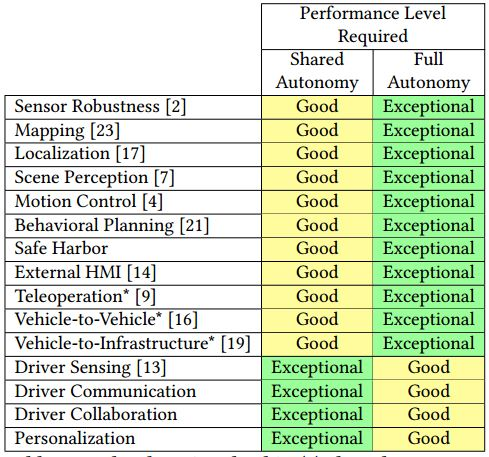
\includegraphics[width=0.45\columnwidth]{pictures/reqTableLexFridman.jpg}
	\caption{Erforderliche Technologien und ihr 'Level' in Stufe 4 \& 5 Fahrzeugen.
		Hier muss ich die Tabelle nochmal selber machen und Quellen aktuell halten.}
	\label{img:fridman1}
\end{figure}

\textbf{Richtlinie 2: Von aufgenommenen Daten lernen} \\
Jede in der obigen Tabelle aufgeführte Technologie soll datengesteuert sein und sich selber iterativ mit Hilfe der erfassten Daten selber verbessern können. Durch gutes Mapping der Features innerhalb eines Autos zueinander ist es möglich, hiervon Datensets für betreutes Lernen zur kreieren. \label{sec:rl2}Dank dieses sich immer wiederholenden Prozesses können Autos in der Zukunft selber von aufgenommenen Daten lernen und sich somit besser dem Fahrer anpassen.\\

\textbf{Richtlinie 3: Fahrerbeobachtung}\\
Bis auf wenige Ausnahmen nutzt kaum ein Unternehmen interne Kameras zum Deuten von Nutzergesten und Beobachten der Fahreraufmerksamkeit. Im Prototypen des HCAV Programms wurden die eben aufgeführten Aspekte von Innenkameras aufgezeichnet und gedeutet. Dadurch kann das Auto mit dem Fahrer kommunizieren wenn es dies als notwendig empfindet. Zu wissen ob der Fahrer abgelenkt, gestresst, müde oder sonstiges ist steigere nicht nur die Fahrsicherheit enorm, sondern unterstützt auch Richtlinie 1 stark.\\

\textbf{Richtlinie 4: Geteilte Wahrnehmungskontrolle}\\
Diese Richtlinie definiert das Ziel, den Status der Systemfähigkeiten und -einschränkungen dem Fahrer stetig zur Verfügung zu stellen. Hierdurch kann dieser das Verhalten des Autos mitverfolgen und Up-to-date mit der Auto-Umwelt bleiben wodurch die Sicherheit bei einer Übernahme des Fahrers gesteigert wird.\\
Auch hier wird stetig von aufgenommenen Daten gelernt, um so bspw. die Lenkart des Fahrers zu imitieren. \textit{\hyperref[sec:rl2]{siehe: Richtlinie 2}}
\\

\textbf{Richtlinie 5: Fahrzeug Personalisierung}\\
Das Auto soll jeden Fahrer einzeln detailliert kennenlernen und sich an diese anpassen wenn sie das Auto betreten. Von Beginn an soll das Auto verschiedene Aspekte des Fahrers kennenlernen(Körpersprache, Mimik, Gestik, Sprachgebrauch,Fahrweise, etc.). Somit ist nach bereits kurzer Zeit jede Konfiguration für Fahrer einzigartig und somit höchst personalisiert.
\\

\textbf{Richtlinie 6: Unvollkommenes Design}\\
Ein Auto soll nicht zur Perfektion streben, sondern Fehler/Schwierige Situationen geeignet Kommunizieren. Durch das Erkennen solcher Situationen gewinnt das Auto nach Auswertung einen hohen Mehrwert. Wichtig ist auch, dass der Fahrer über diese informiert wird. Die bis jetzt beste Art dies zu tun, ist dem Fahrer die Umwelt aus Sicht des Autos zu zeigen(Fig. 2).
\begin{figure}[H]
	\centering
	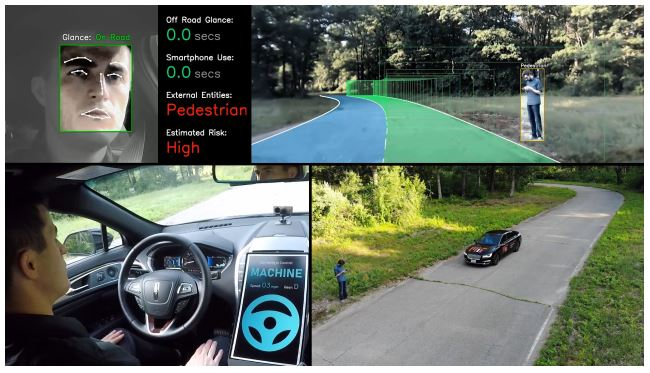
\includegraphics[width=0.734\columnwidth]{pictures/CarView.jpg}
	\caption{Erforderliche Technologien und ihr 'Level' in Stufe 4 \& 5 Fahrzeugen.
		Hier muss ich die Tabelle nochmal selber machen und Quellen aktuell halten.}
	\label{img:CarView}
\end{figure}

\textbf{Richtlinie 7: System-Level Experience}\\
Da weder Fahrzeuge noch Menschen perfekt sind, müssen die Fehler ausgewertet werden um zu Versuchen, daraus zu lernen. Dies soll nicht nur Fahrsicherheitsaspekte betreffen, sondern auch Fehler die im Rahmen Vergnügungsfeatures aufgetreten sind.

\clearpage